%% 
%%	This is file 'beamer_sample.tex'
%%	according to an MPIDR's PowerPoint template (?)
%%	
%%	by Eric Naujoks
%%
%%	Problems, bugs and comments to 
%%	naujoks@demogr.mpg.de
%%

%%%%%%%%%%%%%%%%%%%%%%%%%%%%%%%%%%
%%	Praelegomena								%%
%%%%%%%%%%%%%%%%%%%%%%%%%%%%%%%%%%
%%	- Make sure that you use utf8-encoding for all your .tex-files!!! (TeXnicCenter since version 2.0)
%%	- TeXnicCenter update: MPIDR intranet > Hard- & Sortfware > Software > Script and text editors > TeXnicCenter

\documentclass[20pt]{beamer}

\usepackage[ngerman,english]{babel}
\usepackage{tikz}
\usepackage[normalem]{ulem}
\geometry{paperwidth=10in, paperheight=7.5in}
\usepackage{animate}
\usepackage{array}

\usepackage[utf8]{inputenc}

\usepackage[mpidr]{./mpidr/beamerthemeMPIDR}
\newcommand{\dd}{\; \mathrm{d}}
\newcommand{\scen}[1]{\includegraphics[scale=.8]{Figures/scenarios/{scenario#1}.pdf}}
\newcolumntype{C}{ >{\centering\arraybackslash} m{10cm} }
\newcolumntype{D}{ >{\centering\arraybackslash} m{1.5cm} }
%% Declaring title and author
\title{Morbidity concentration and dispersion}
\subtitle{\small{Tim Riffe, 
A{\"i}da Sol\'{e} Auro, 
Maarten J. Bijlsma}
}		%%

%%	the institute's logo
\renewcommand{\mylogo}{\includegraphics[width=4.7in]{mpidr_logo_colour_en}}
\usepackage{color}
\definecolor{mygray}{rgb}{0.8,0.8,0.8}

\defbeamertemplate{description item}{align left}{\insertdescriptionitem\hfill}
%%	should be the very last package to be loaded
\usepackage{hyperref}

%%%%%%%%%%%%%%%%%%%%%%%%%%%%%%%%%%
%%	Beginning of the document		%%
%%%%%%%%%%%%%%%%%%%%%%%%%%%%%%%%%%
\begin{document}

%%	titlepage - fixed frame:
%%	========================

\begin{frame}
	\titlepage
\end{frame}
%-------------------

\begin{frame}
\frametitle{Fries' diagrams are a nice prop}
\begin{center}
  \begin{tikzpicture}
    \node<1> (img1)
    {\includegraphics[width=.8\linewidth]{Figures/FriesFigure1.pdf}}; 
  \end{tikzpicture}
\end{center}
\end{frame}


\begin{frame}
\frametitle{Pattern indifference within lifespan}
\begin{center}
  \begin{tikzpicture}
    \node<1> (img1)
    {
\includegraphics[width=.9\linewidth]{Figures/boxflip1.pdf}}; 
    \node<2>
    (img2) {
\includegraphics[width=.9\linewidth]{Figures/boxflip2.pdf}}; 
  \end{tikzpicture}\\ \vspace{5cm}

\end{center}

\end{frame}
\begin{frame}
\frametitle{Patterns matter if lifespans are mixed}
\begin{center}
  \begin{tikzpicture}
    \node<1> (img1)
    {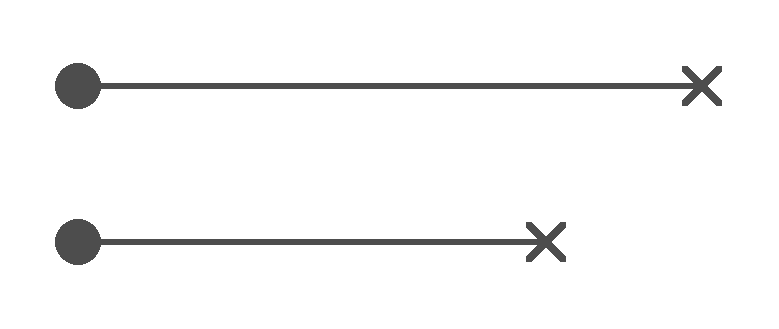
\includegraphics[width=.7\linewidth]{Figures/lifelines1.pdf}}; 
    \node<2>
    (img2) {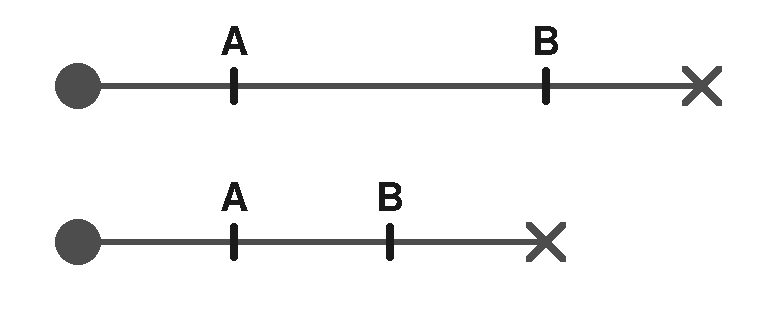
\includegraphics[width=.7\linewidth]{Figures/lifelines2.pdf}}; 
    \node<3> (img3) {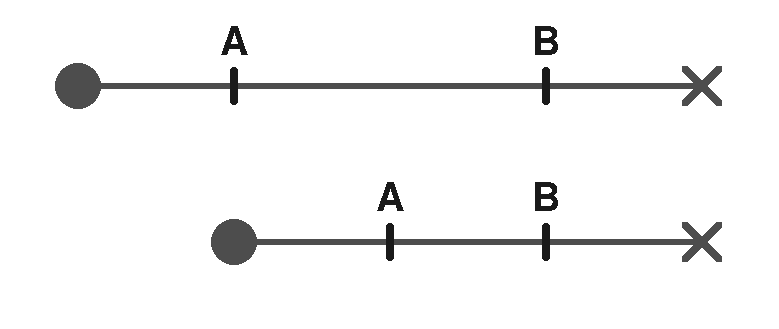
\includegraphics[width=.7\linewidth]{Figures/lifelines3.pdf}};
  \end{tikzpicture}
\end{center}
\end{frame}


\begin{frame}
\frametitle{Patterns matter if lifespans are mixed}
\begin{center}
  \begin{tikzpicture}
    \node<1> (img1)
    {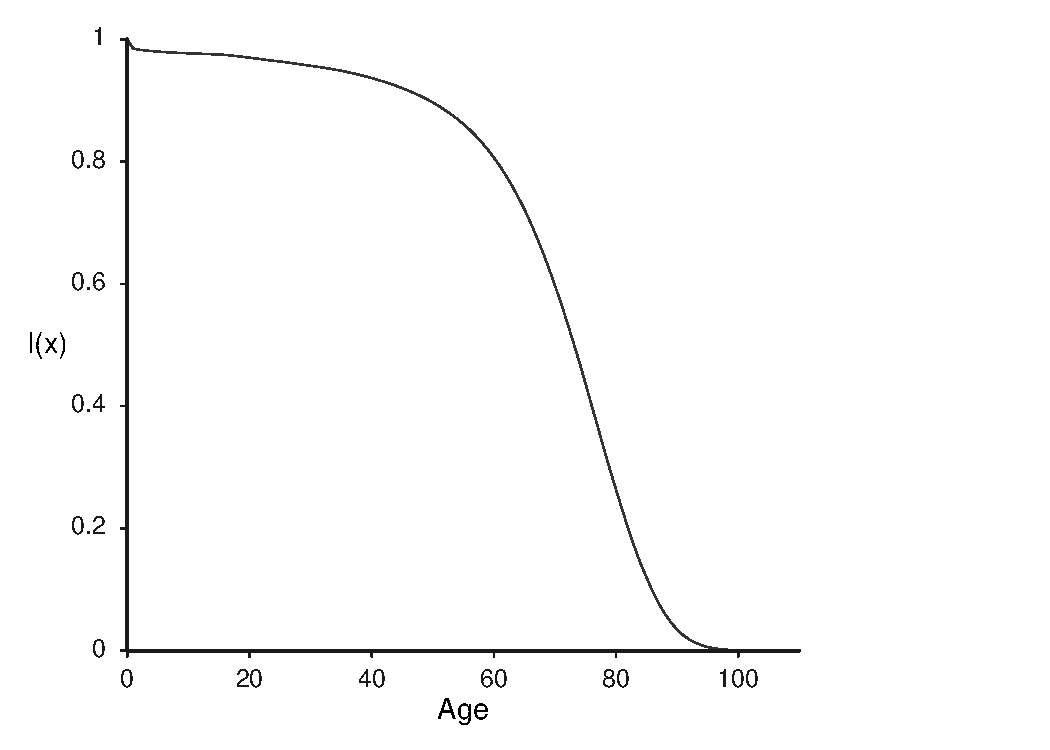
\includegraphics[width=.9\linewidth]{Figures/Japan1.pdf}}; 
    \node<2>
    (img2) {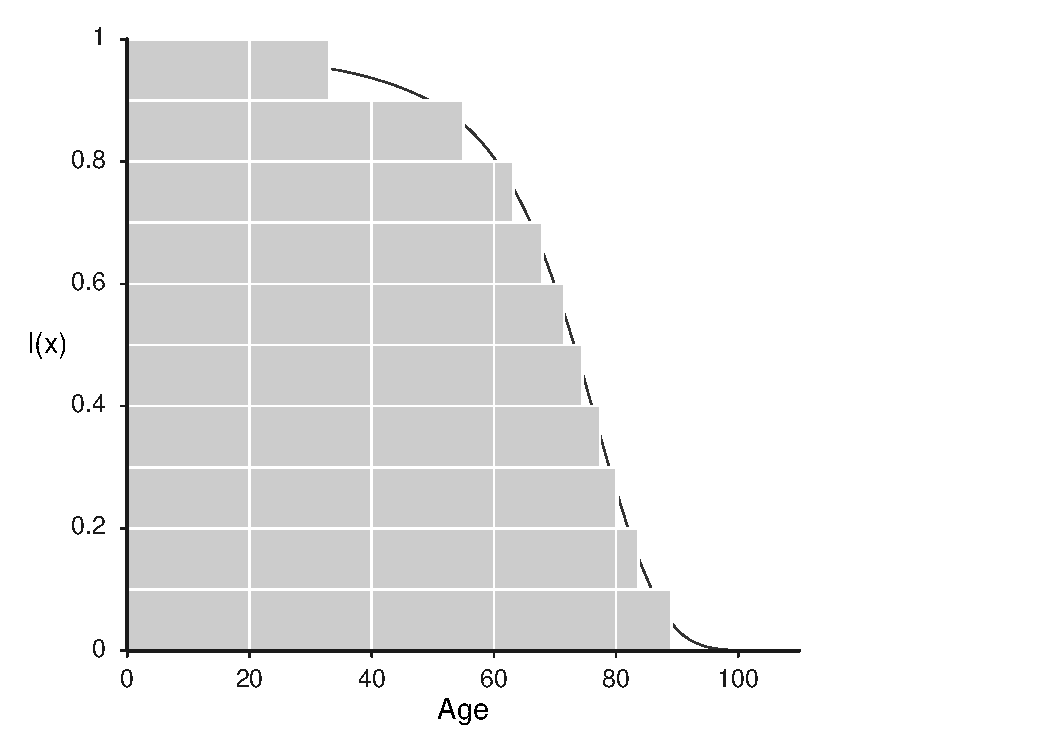
\includegraphics[width=.9\linewidth]{Figures/Japan2.pdf}}; 
     \node<3>
    (img3) {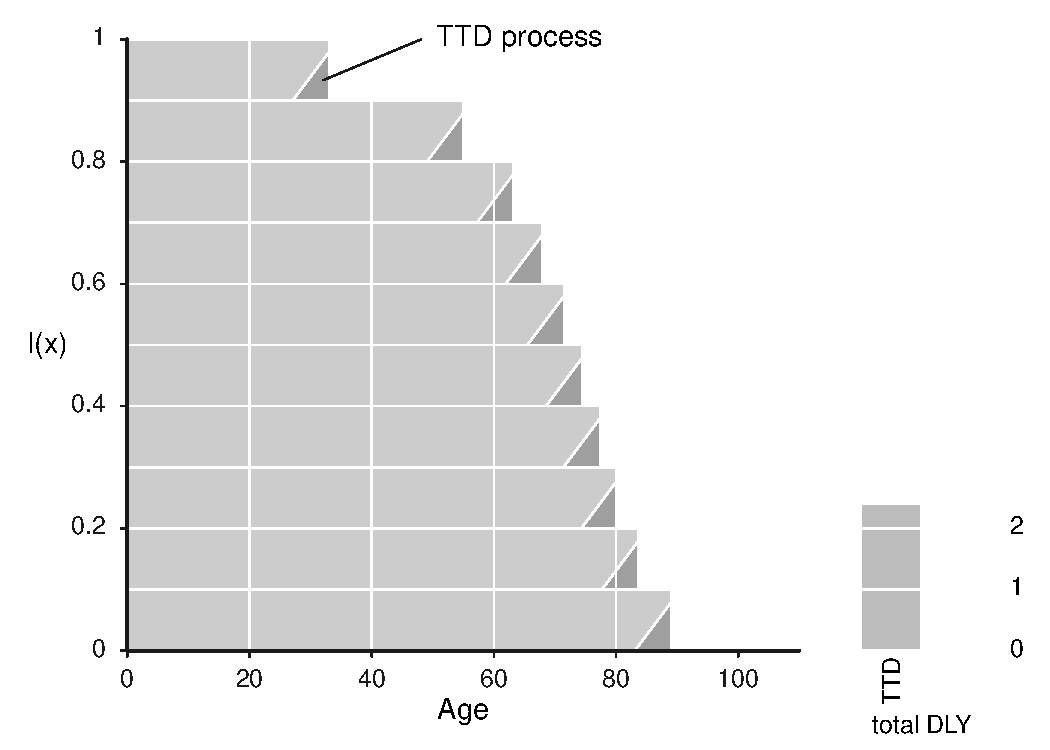
\includegraphics[width=.9\linewidth]{Figures/Japan3.pdf}}; 
    % \node<4>
   % (img4) {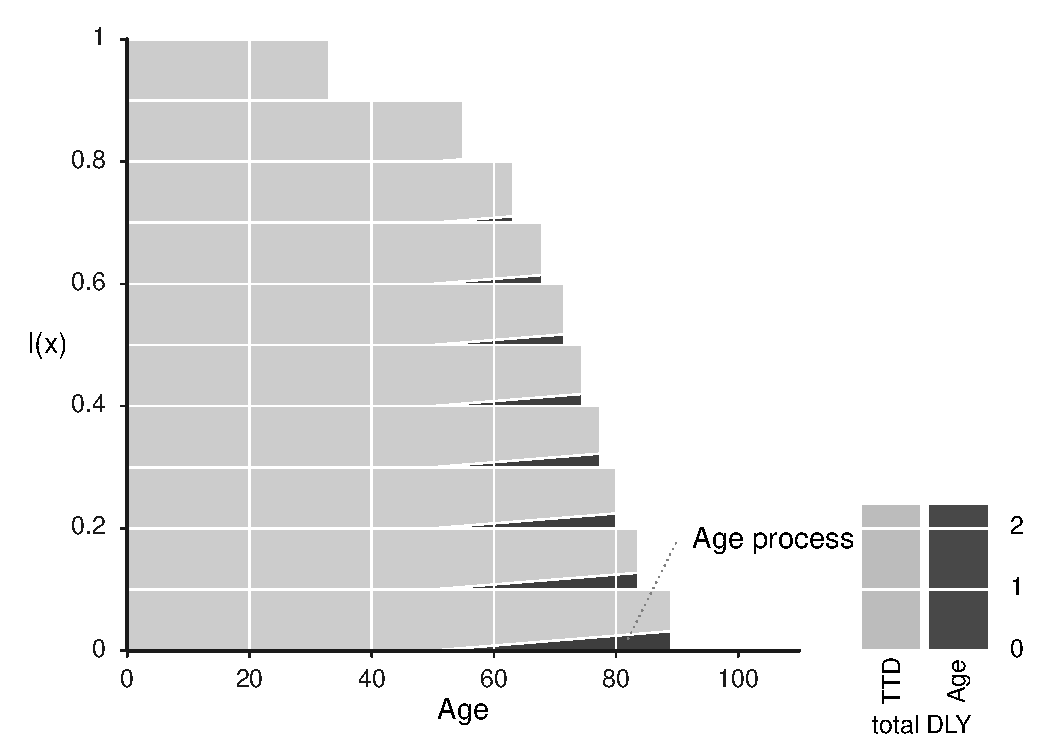
\includegraphics[width=.9\linewidth]{Figures/Japan4.pdf}}; 
     \node<4>
    (img4) {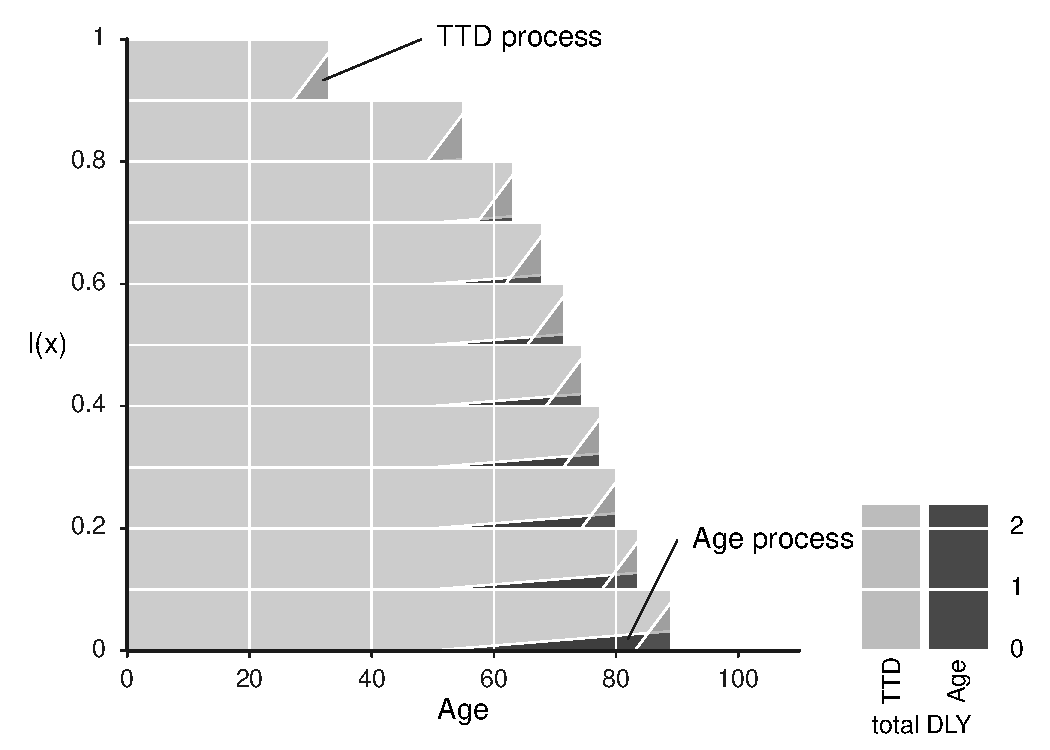
\includegraphics[width=.9\linewidth]{Figures/Japan5.pdf}}; 
     \node<5>
    (img5) {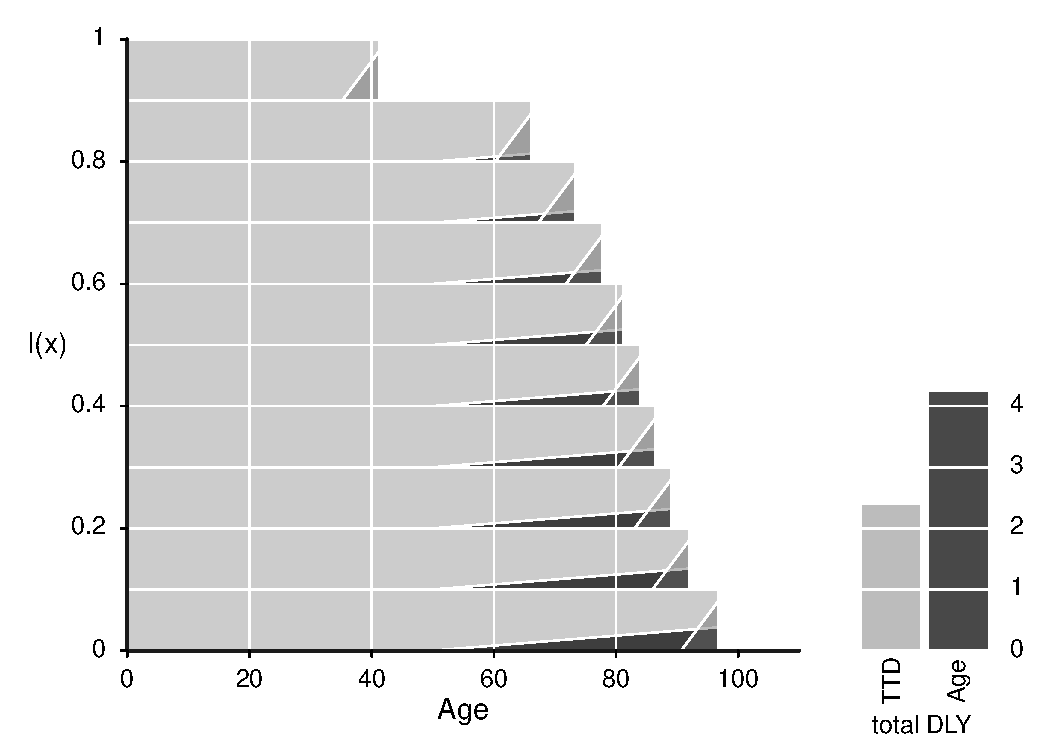
\includegraphics[width=.9\linewidth]{Figures/Japan6.pdf}}; 
  \end{tikzpicture}
\end{center}
\end{frame}

\begin{frame}
\frametitle{Compression}
\begin{block}{Compression definition}
The level of morbidity compression is the average proportion of life in good
health, $\mathbb{C} = \frac{HLE}{LE}$.
\end{block}


\pause
\begin{block}{Objective:}
Separate morbidity levels and morbidity dispersion.
\end{block}
\end{frame}

\begin{frame}
\frametitle{Dispersion}
\begin{block}{Dispersion definition}
Morbidity dispersion, $\mathbb{D}$, is the average time-to-death of late-life
morbidity prevalence.
\end{block}
\pause

\begin{block}{Formal definition}
\begin{equation}
\mathbb{D} = \frac{\int_0^{\omega} y \pi^\star(y) \dd
y}{\int_0^{\omega}\pi^\star(y)\dd y}
\end{equation}
where $a$ is age, $y$ is time until death, and $\pi^\star(y)$ is morbidity
prevalance by time to death.
\end{block}

\pause
Or one might rather weight a lifespan-varying $\pi(y,l)$, by the length-of-life
distribution.

\end{frame}

\begin{frame}
\frametitle{Scenarios}
\begin{tabular}{D C D D D D D}
~ & Scenario & $ULE$ & $HLE$ & $LE$ & $\mathbb{C}$ & $\mathbb{D}$ \\
\hline
Base & \scen{1} & ~ & ~ & ~ & ~ & ~ \\
\only<1>{ & \scen{0} & ~ & ~ & ~ & ~ & ~ \\}
\only<2>{ & \scen{2} & $=$ & $=$ & $=$ & $=$ & $\downarrow$ \\}
\only<3>{ & \scen{8} & $=$ & $=$ & $=$ & $=$ & $\uparrow$ \\}
\only<4>{ & \scen{3} & $\downarrow$ & $\uparrow$ & $=$ & $\uparrow$ &  $=$ \\}
\only<5>{ & \scen{9} & $\downarrow$ & $\uparrow$ & $=$ & $\uparrow$ & 
$\downarrow$ \\} 
\only<6>{ & \scen{4} & $\uparrow$ & $\downarrow$ & $=$ & $\downarrow$ &  $=$ \\}
\only<7>{ & \scen{5} & $=$ & $\uparrow$ & $\uparrow$ & $\uparrow$ &  $=$ \\}
\only<8>{ & \scen{6} & $\uparrow$ & $\uparrow$ & $\uparrow$ & $\downarrow$ & 
$\downarrow$ \\} 
\only<9>{ & \scen{7} & $=$ & $\uparrow$ & $\uparrow$ &  $\uparrow$ &
$\downarrow$\\}
\end{tabular}
\end{frame}
%\begin{frame}
%\frametitle{Fries' diagrams are ignored in practice}
%\begin{center}
%  \begin{tikzpicture}
%    \node<1> (img1)
%    {\includegraphics[width=.8\linewidth]{Figures/FriesFigure1.pdf}}; 
%    \node<2>
%    (img2) {\includegraphics[width=.8\linewidth]{Figures/FriesFigure2.pdf}}; 
%  \end{tikzpicture}
%\end{center}
%\end{frame}

%\begin{frame}
%\frametitle{Schematic time-to-death patterns}
%\vspace{-2em}
%\begin{center}
%  \begin{tikzpicture}
%    \node<1> (img1)
%    {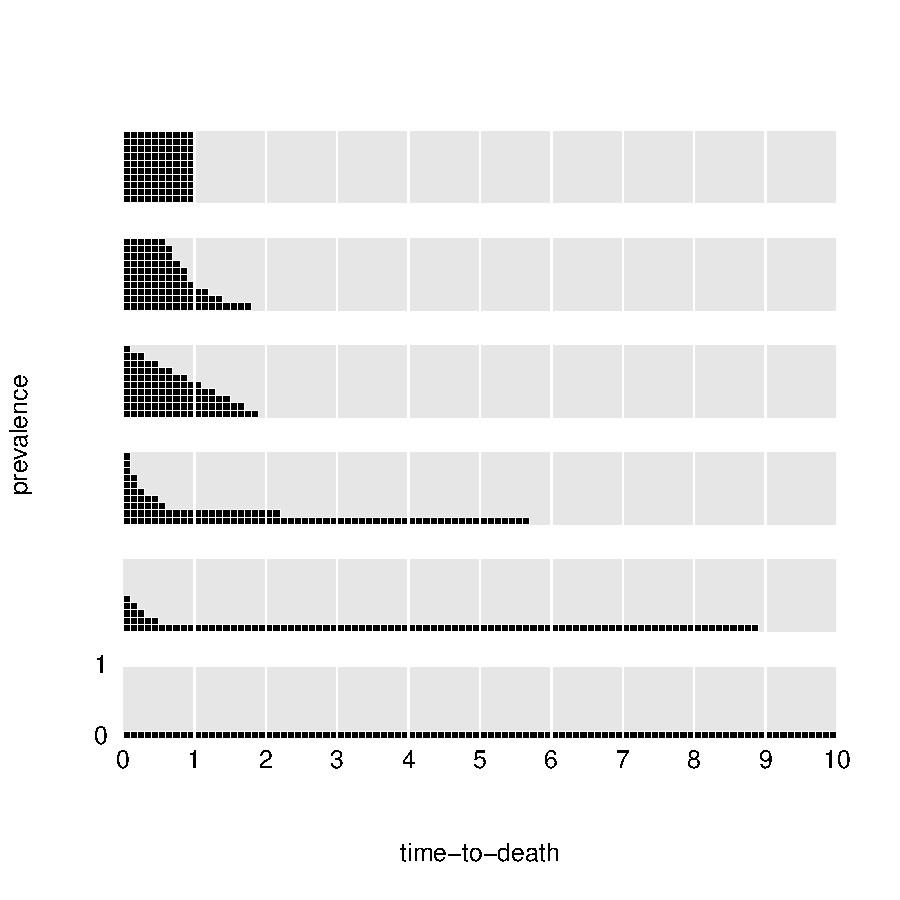
\includegraphics[width=.8\linewidth]{Figures/CompareTTD1.pdf}}; 
%    \node<2>
%    (img2) {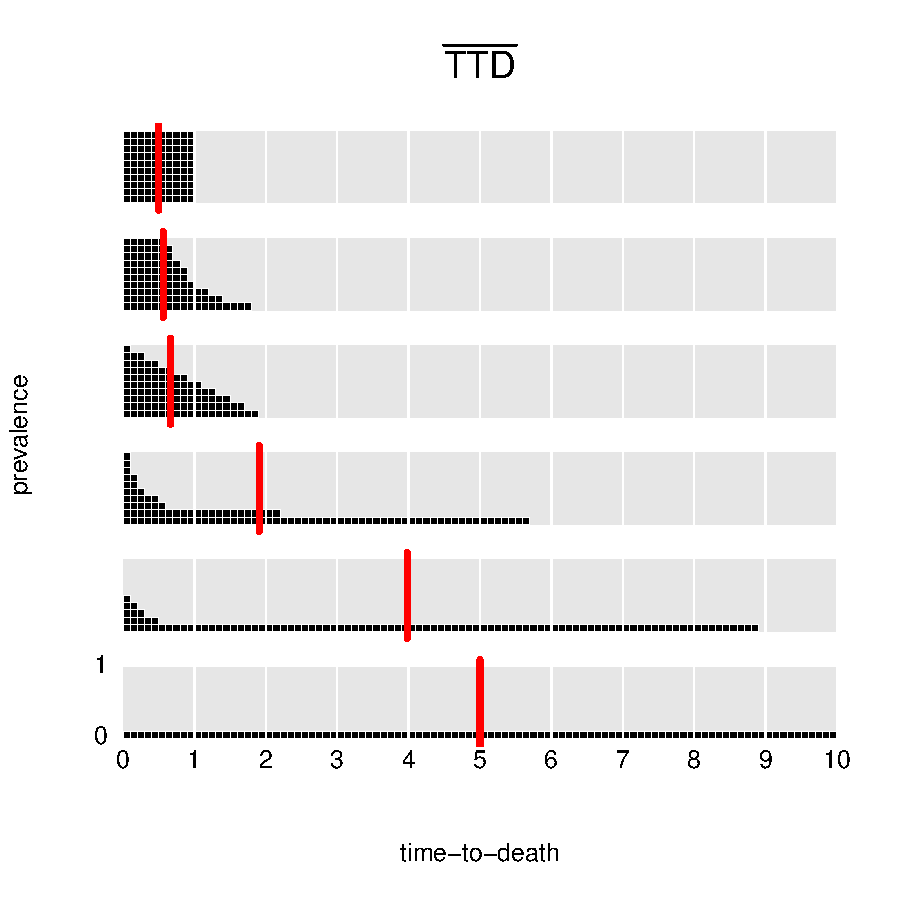
\includegraphics[width=.8\linewidth]{Figures/CompareTTD2.pdf}}; 
%    \node<3>
%    (img3) {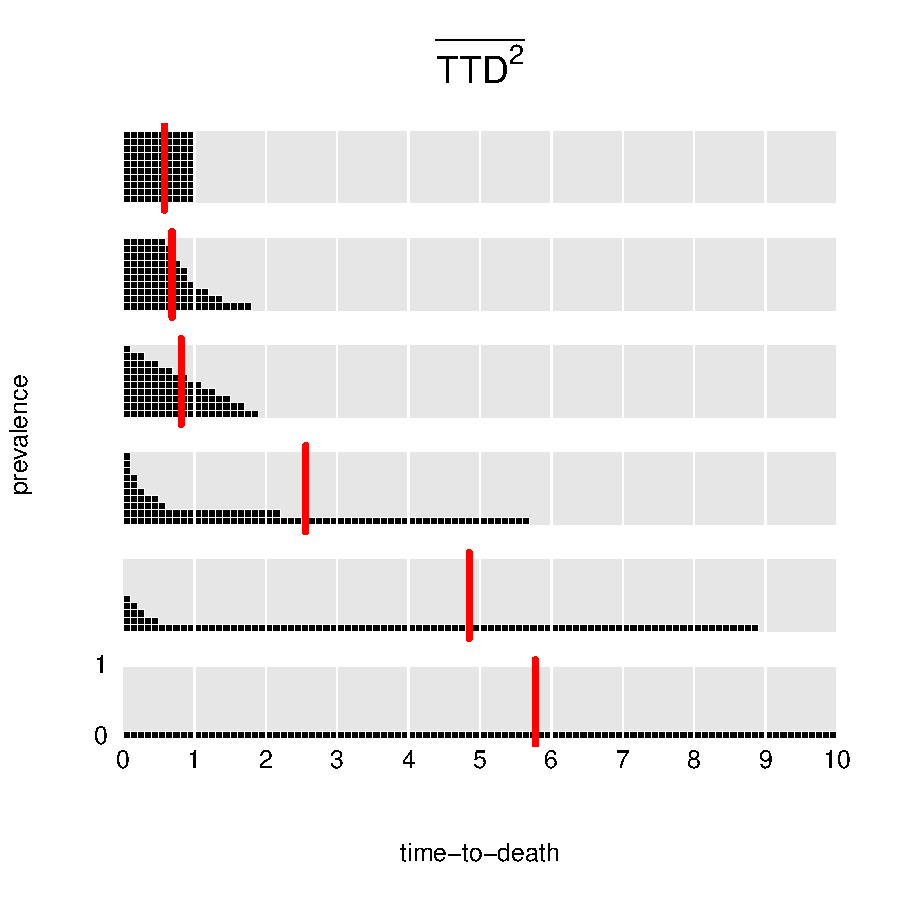
\includegraphics[width=.8\linewidth]{Figures/CompareTTD3.pdf}}; 
%    \node<4>
%    (img4) {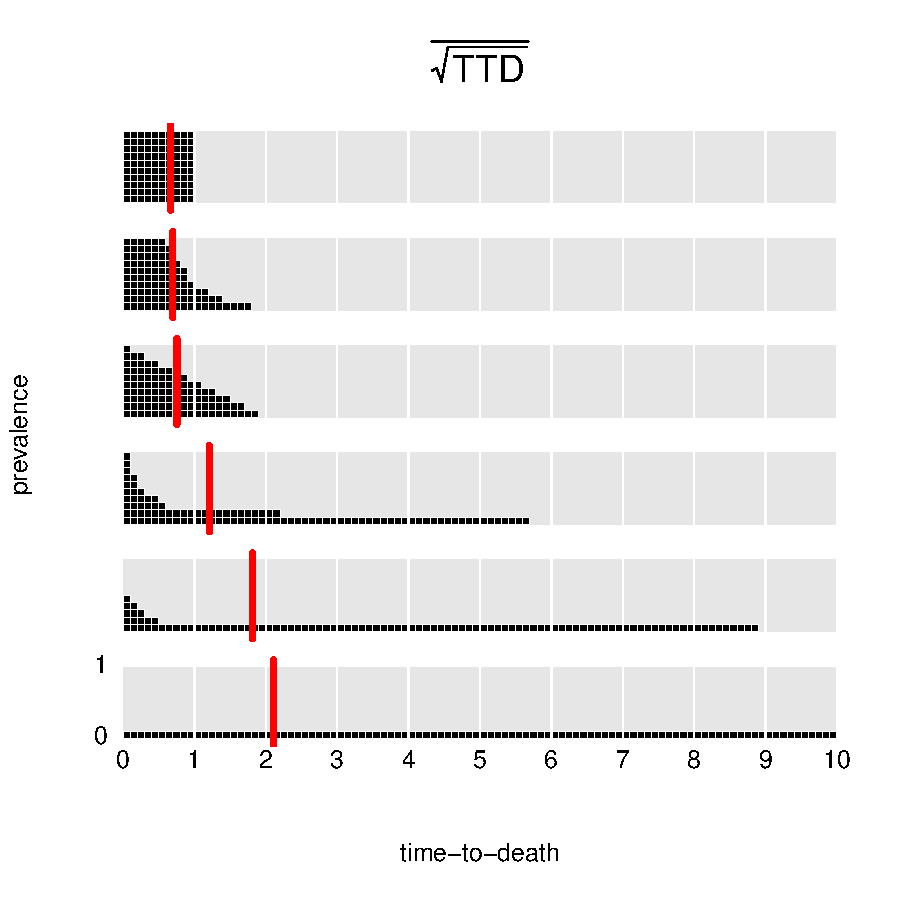
\includegraphics[width=.8\linewidth]{Figures/CompareTTD4.pdf}}; 
%  \end{tikzpicture}
%\end{center}
%\end{frame}

\begin{frame}
\frametitle{Observed time-to-death patterns (HRS, ADL3)}
\vspace{-1em}
\begin{center}
  \begin{tikzpicture}
    \node<1>  (img1) {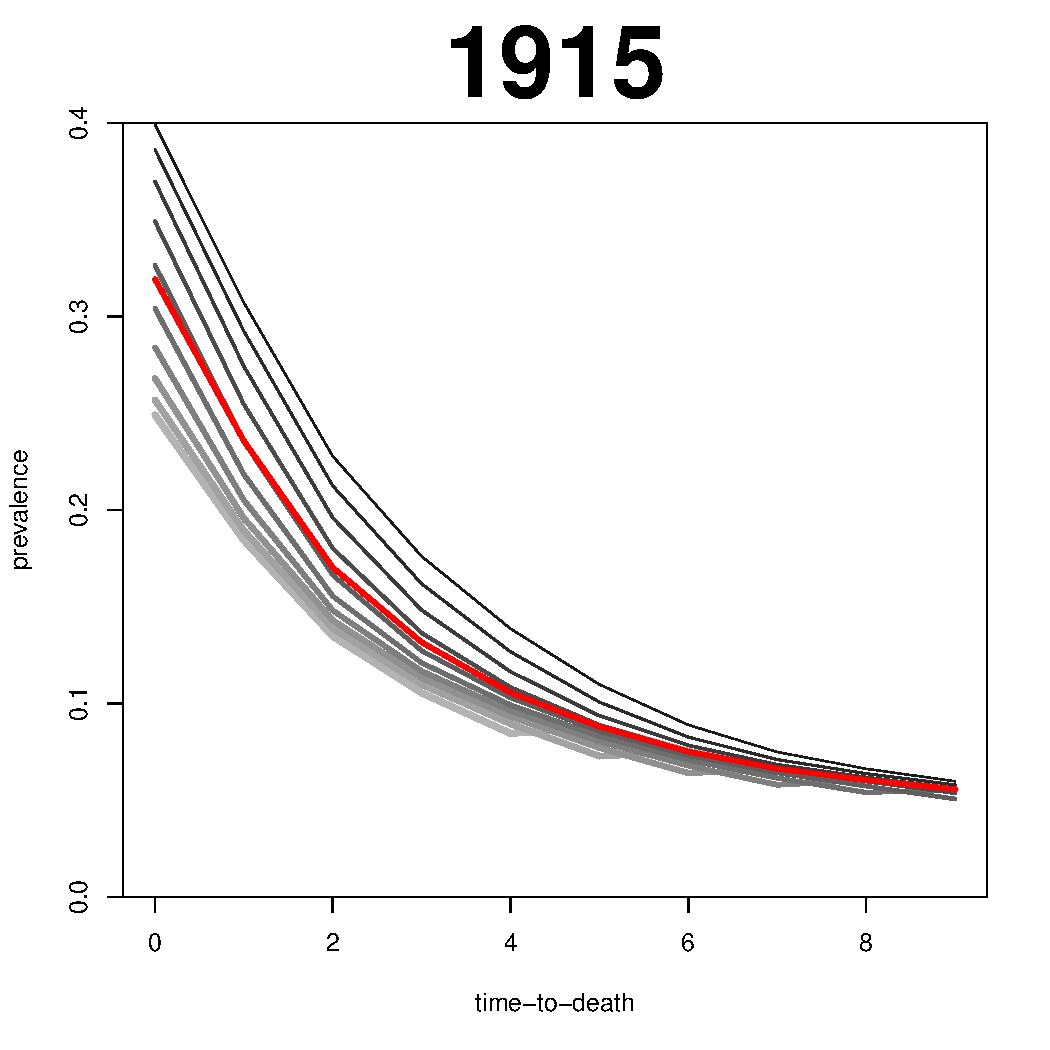
\includegraphics[width=.7\linewidth]{Figures/adl31915.pdf}}; 
    \node<2>  (img2) {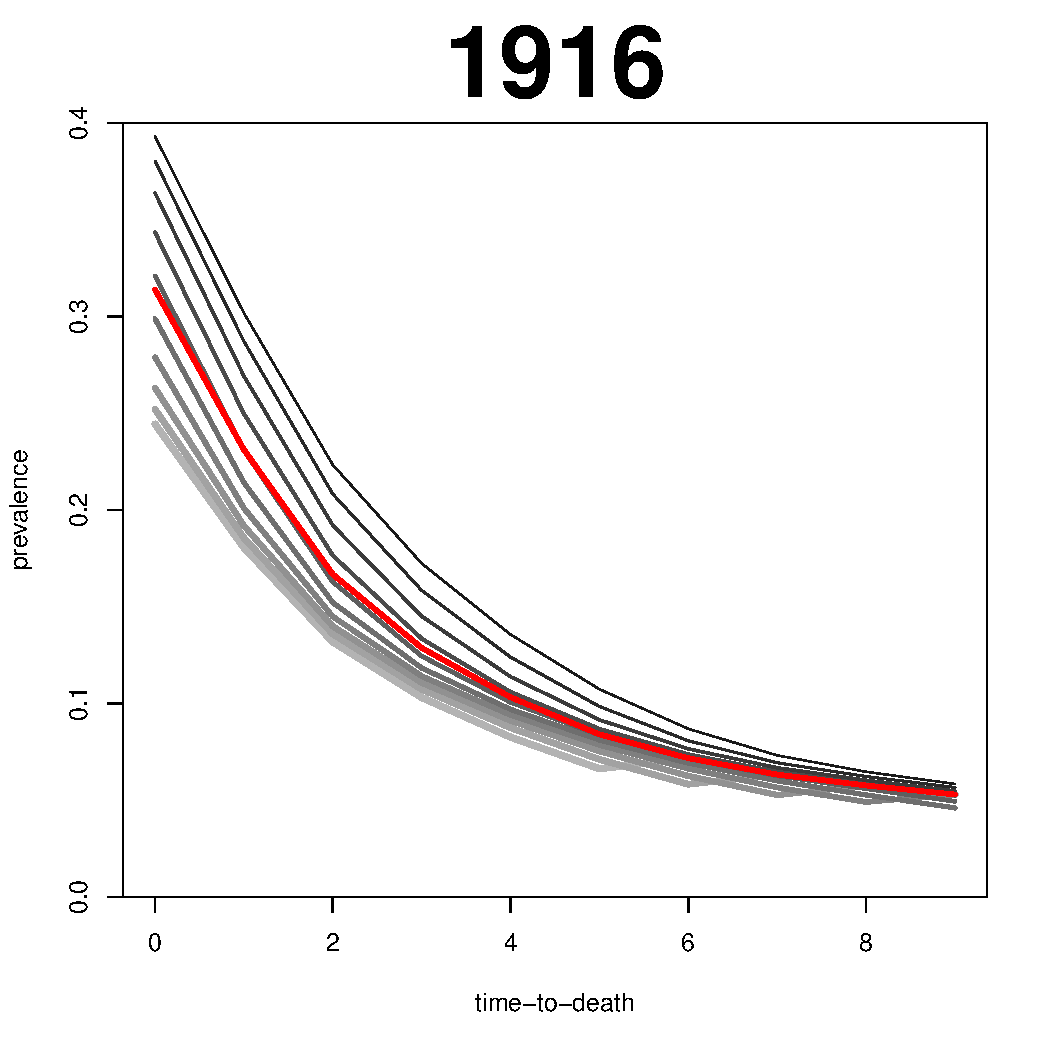
\includegraphics[width=.7\linewidth]{Figures/adl31916.pdf}}; 
    \node<3>  (img3) {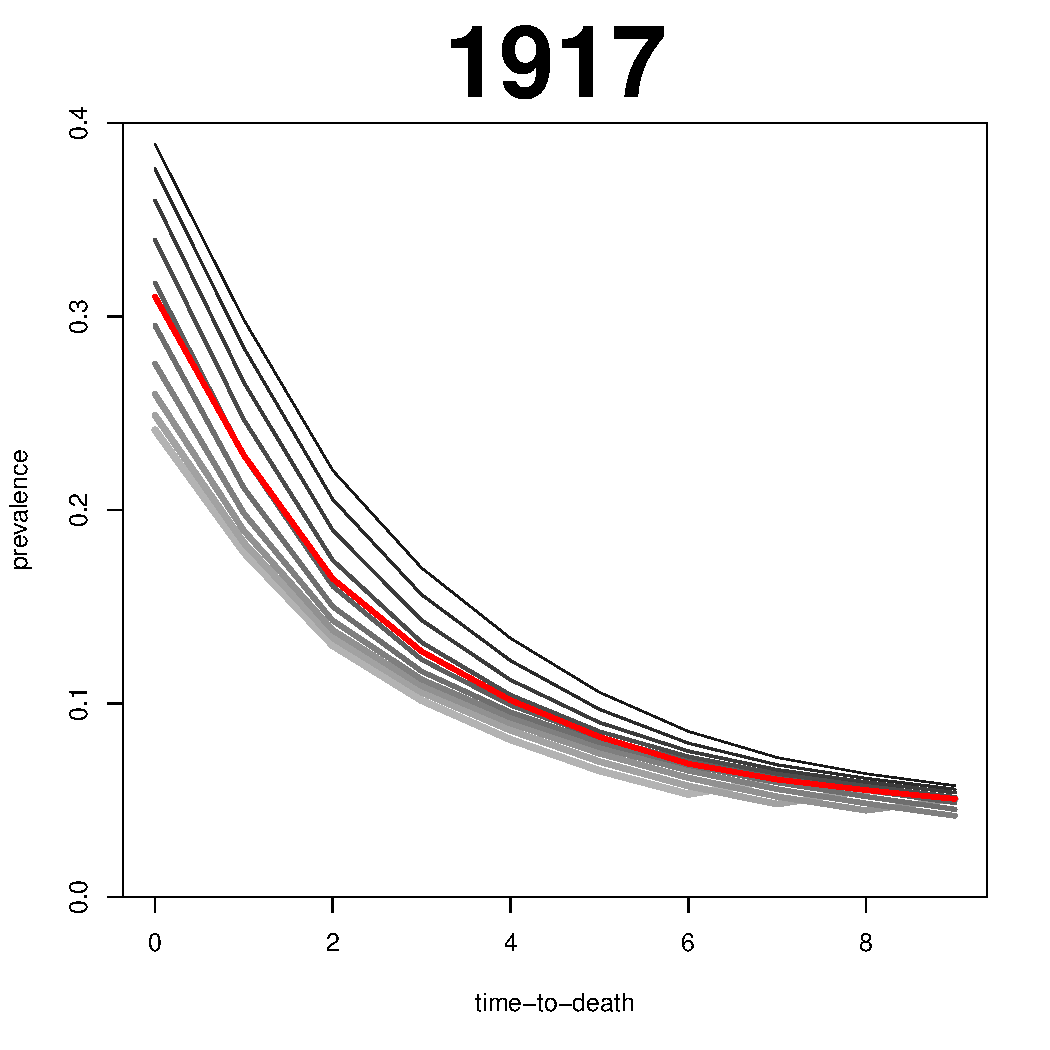
\includegraphics[width=.7\linewidth]{Figures/adl31917.pdf}}; 
    \node<4>  (img4) {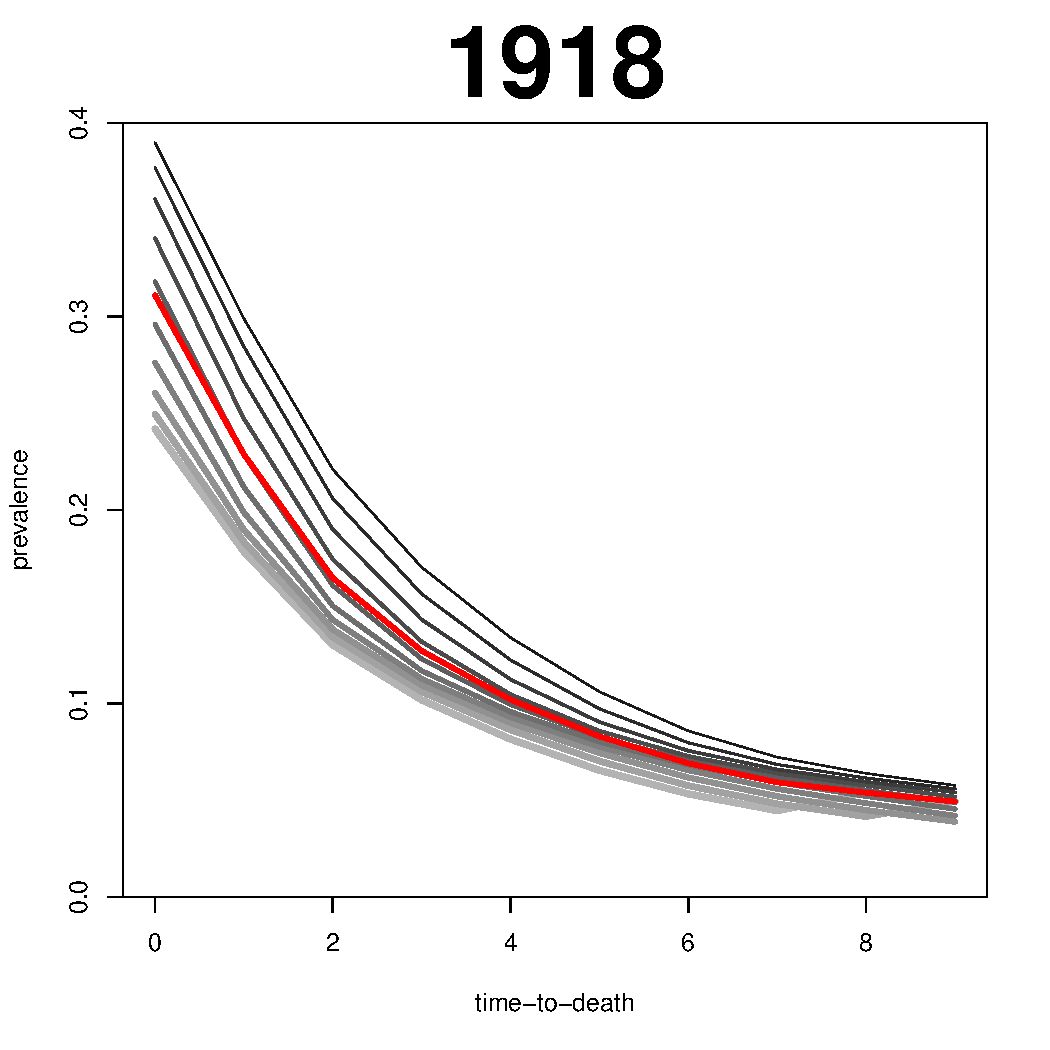
\includegraphics[width=.7\linewidth]{Figures/adl31918.pdf}}; 
    \node<5>  (img5) {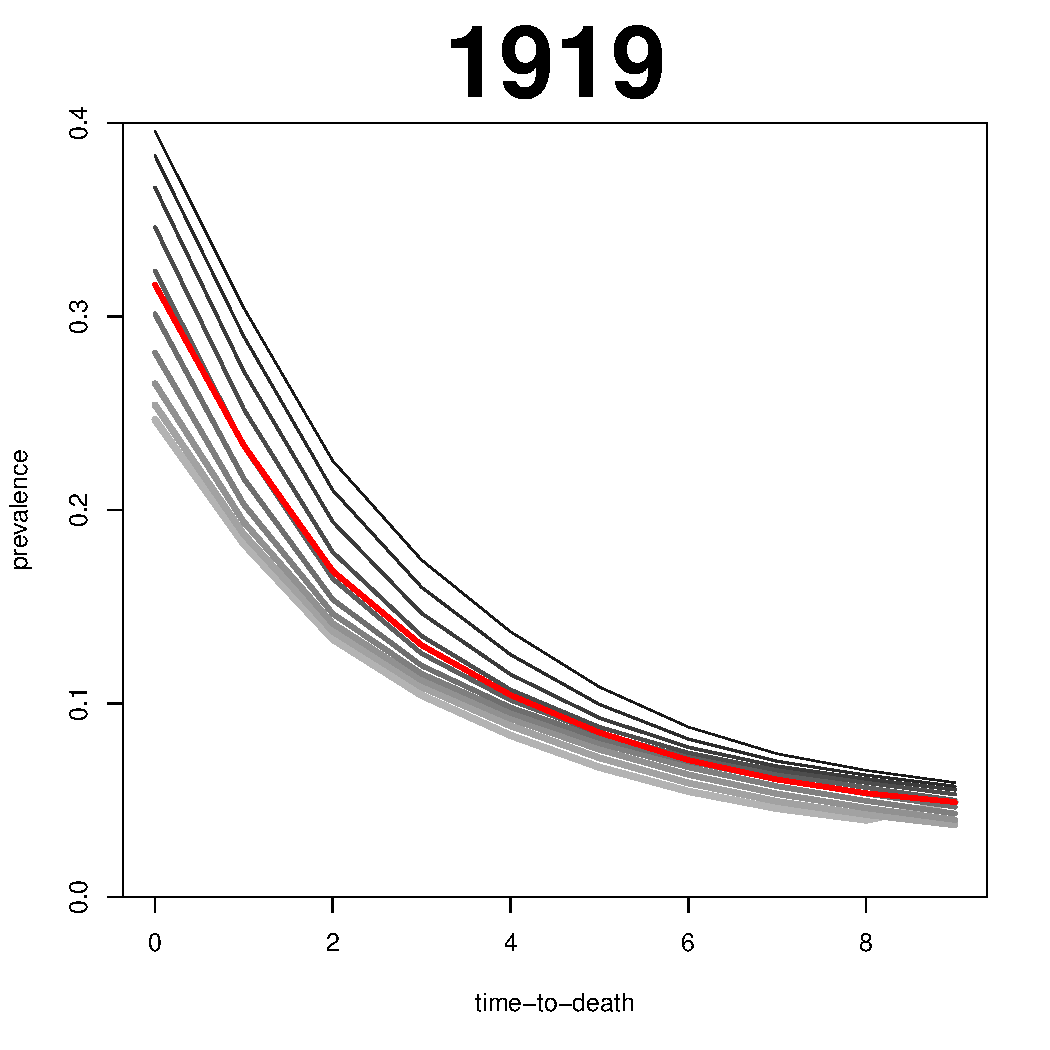
\includegraphics[width=.7\linewidth]{Figures/adl31919.pdf}}; 
    \node<6>  (img6) {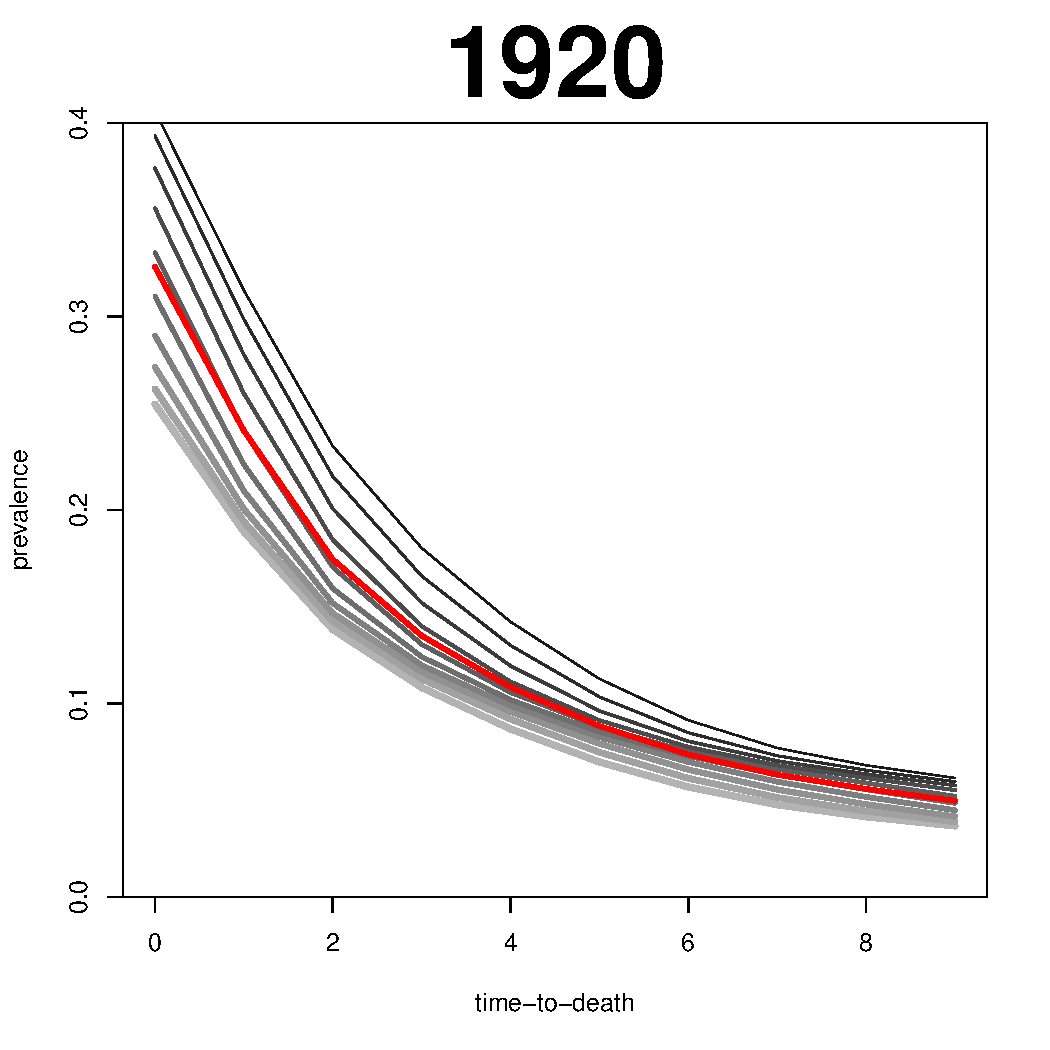
\includegraphics[width=.7\linewidth]{Figures/adl31920.pdf}}; 
    \node<7>  (img7) {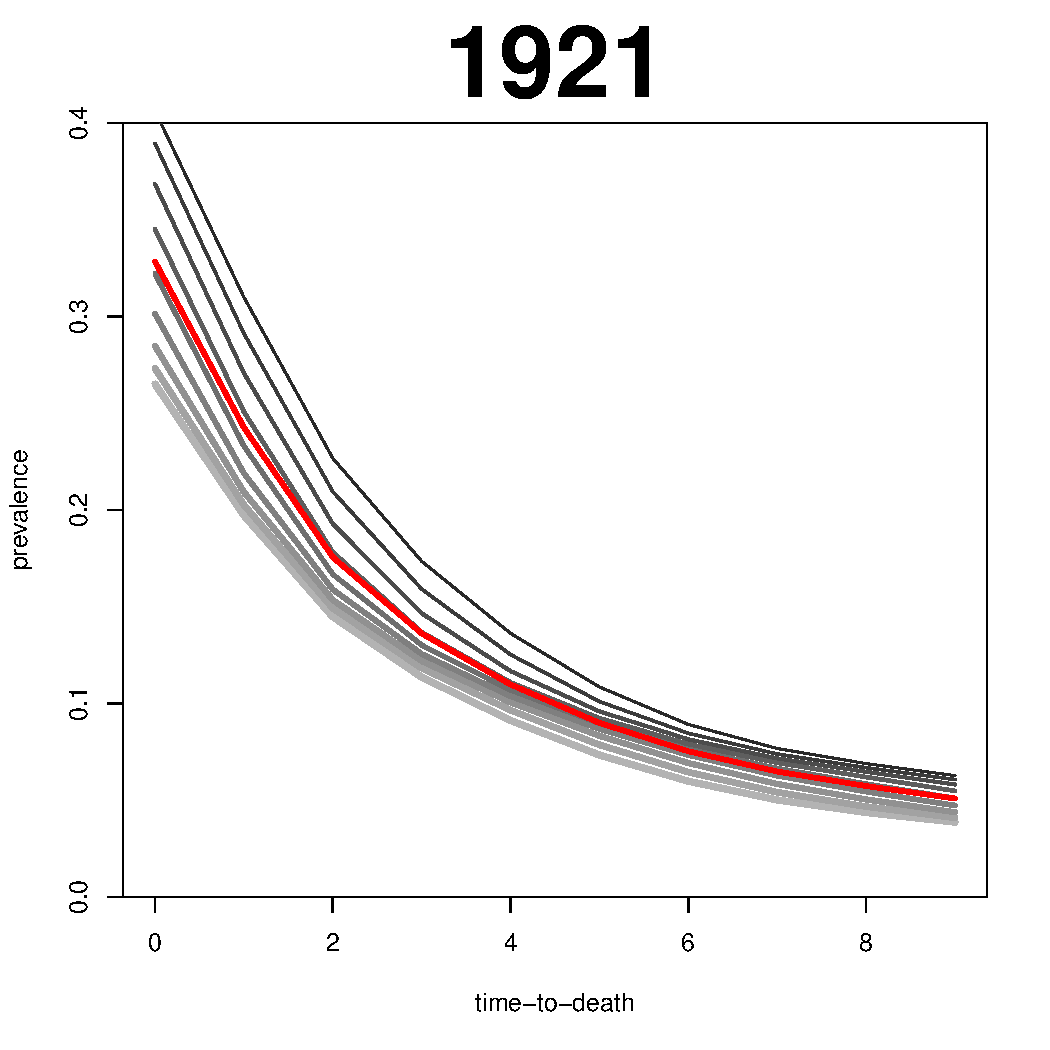
\includegraphics[width=.7\linewidth]{Figures/adl31921.pdf}}; 
    \node<8>  (img8) {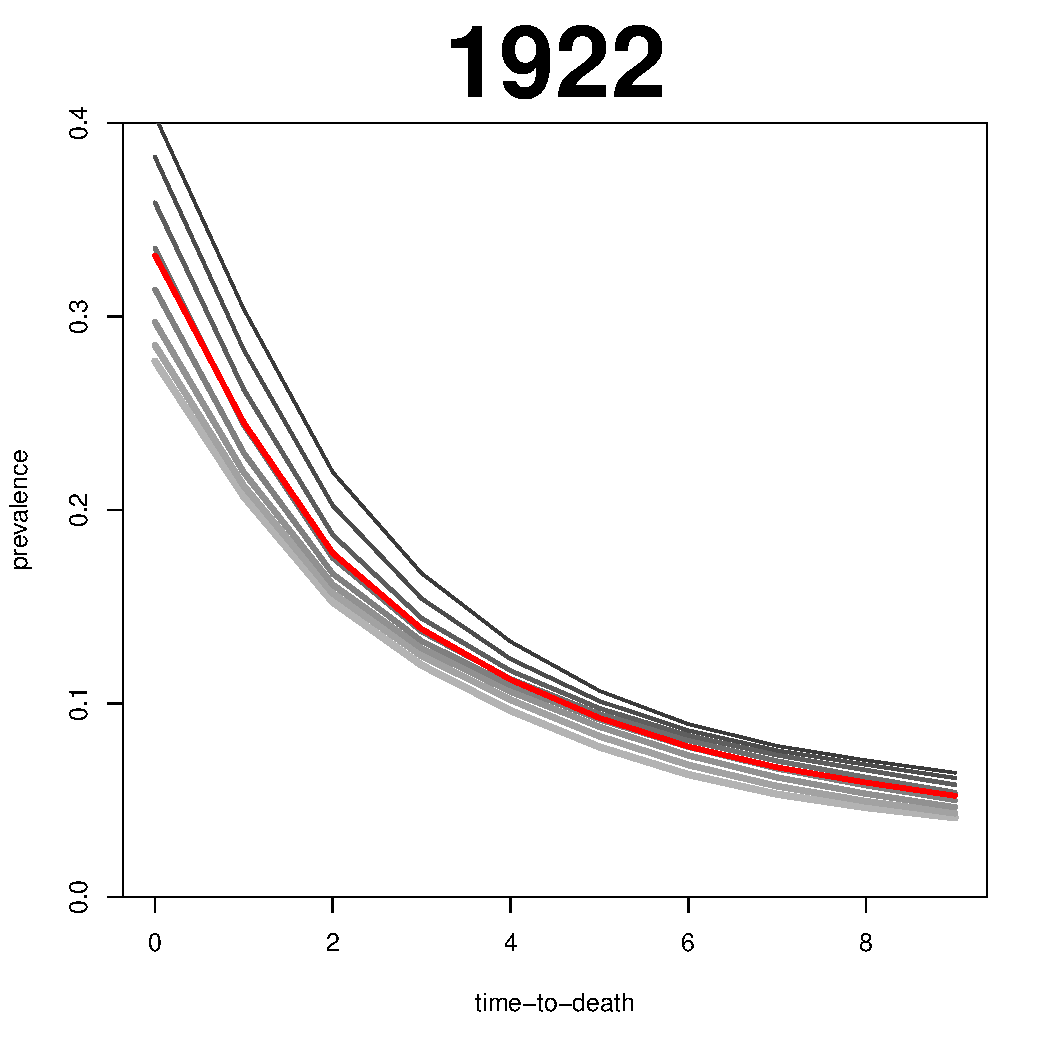
\includegraphics[width=.7\linewidth]{Figures/adl31922.pdf}}; 
    \node<9>  (img9) {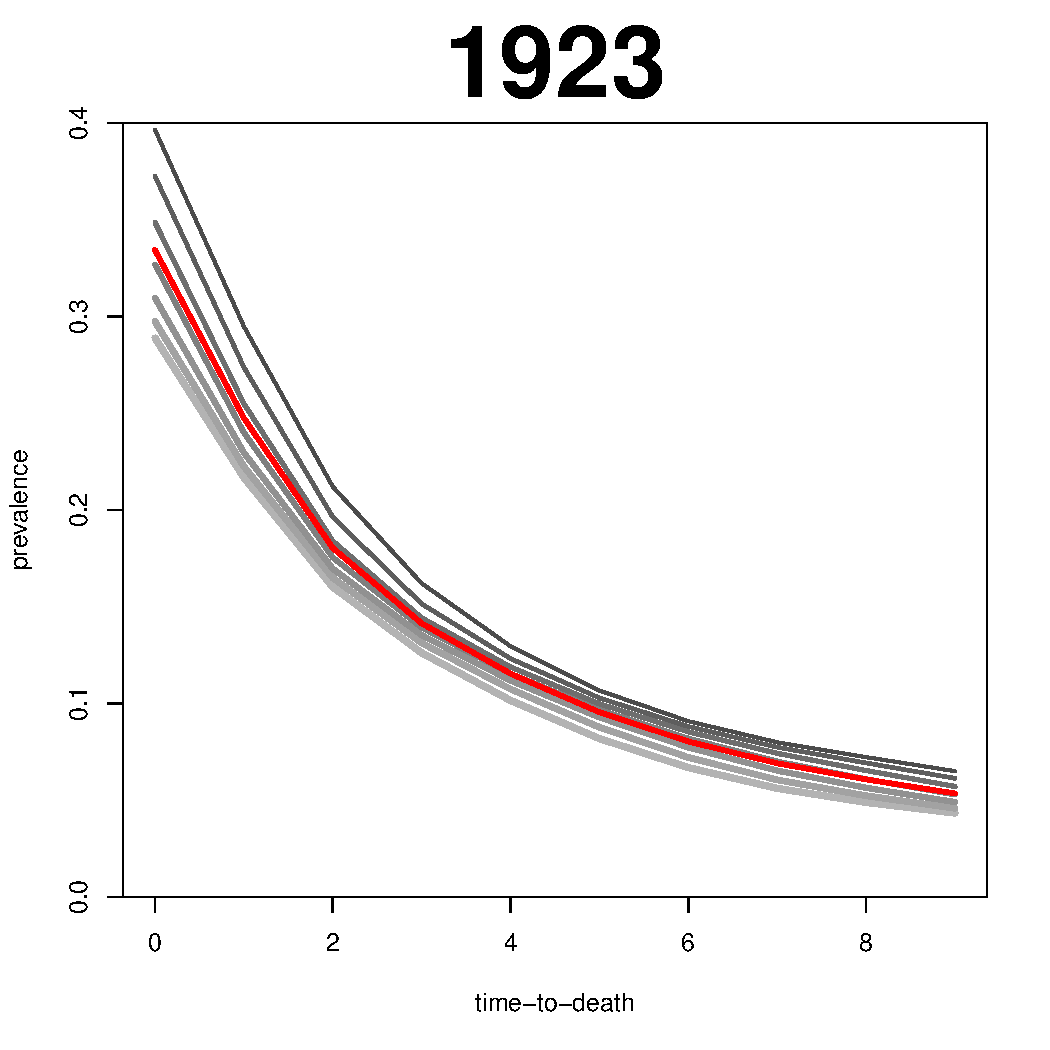
\includegraphics[width=.7\linewidth]{Figures/adl31923.pdf}}; 
    \node<10> (img10) {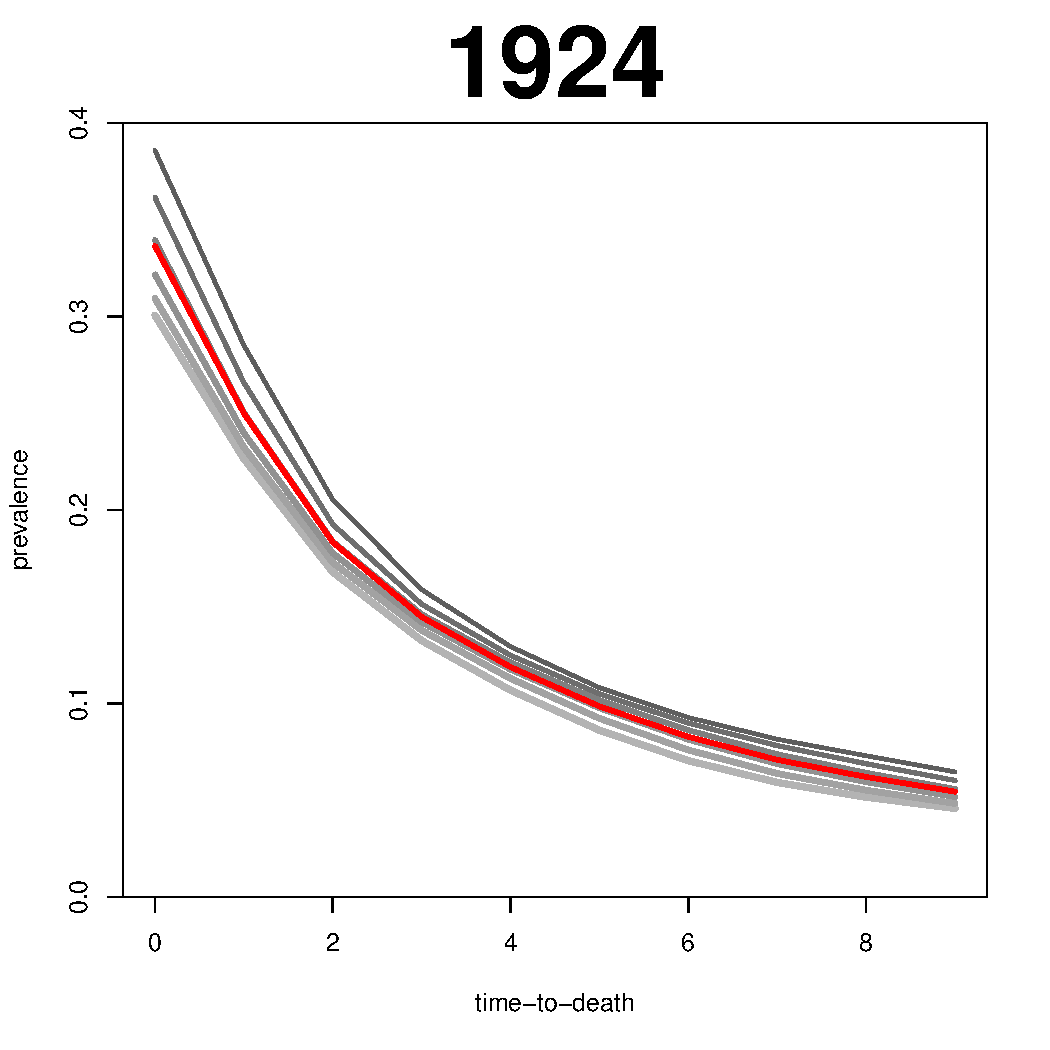
\includegraphics[width=.7\linewidth]{Figures/adl31924.pdf}}; 
    \node<11> (img11) {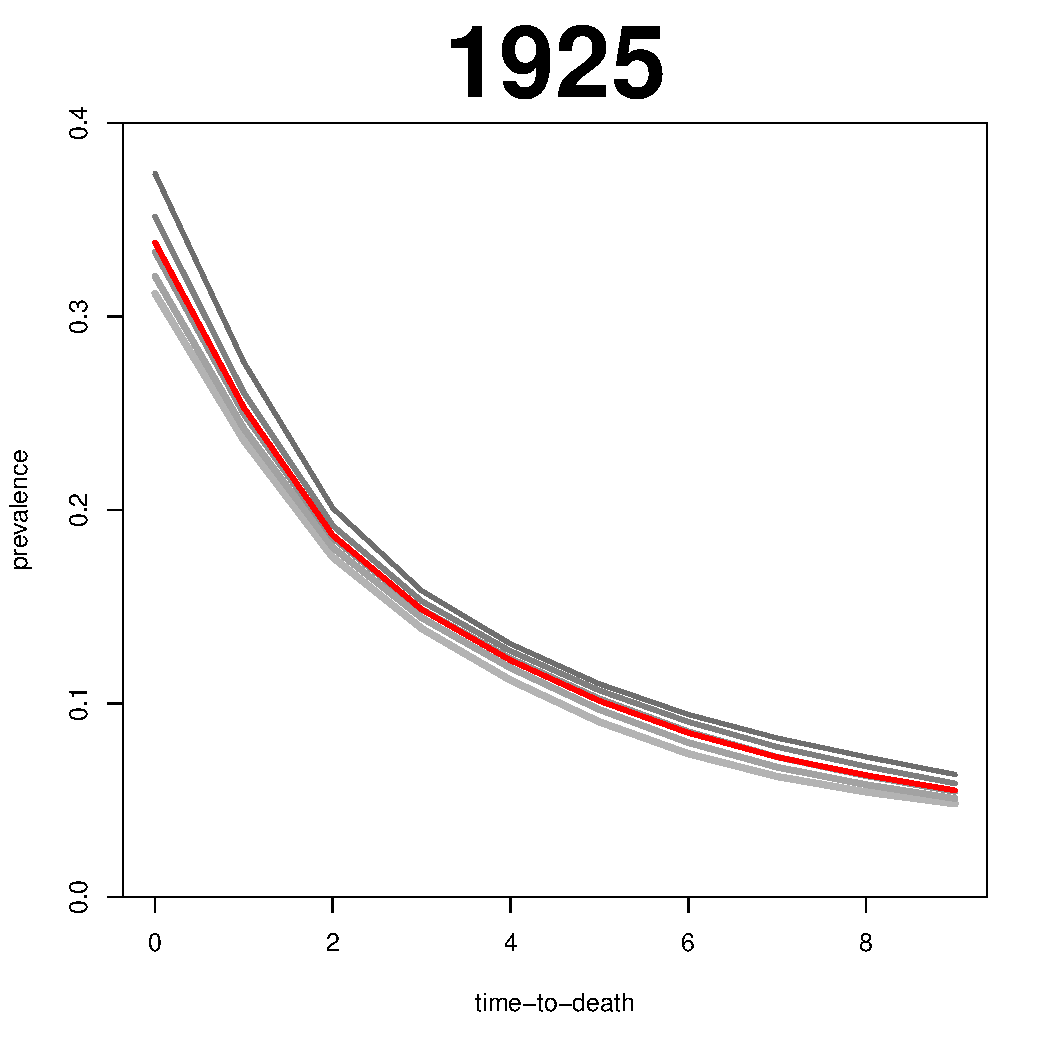
\includegraphics[width=.7\linewidth]{Figures/adl31925.pdf}}; 
  \end{tikzpicture}
\end{center}
\end{frame}

%\begin{frame}
%\frametitle{ \boldmath$\overline{TTD}$ patterns, psych problems and ADL3}
%\begin{center}
%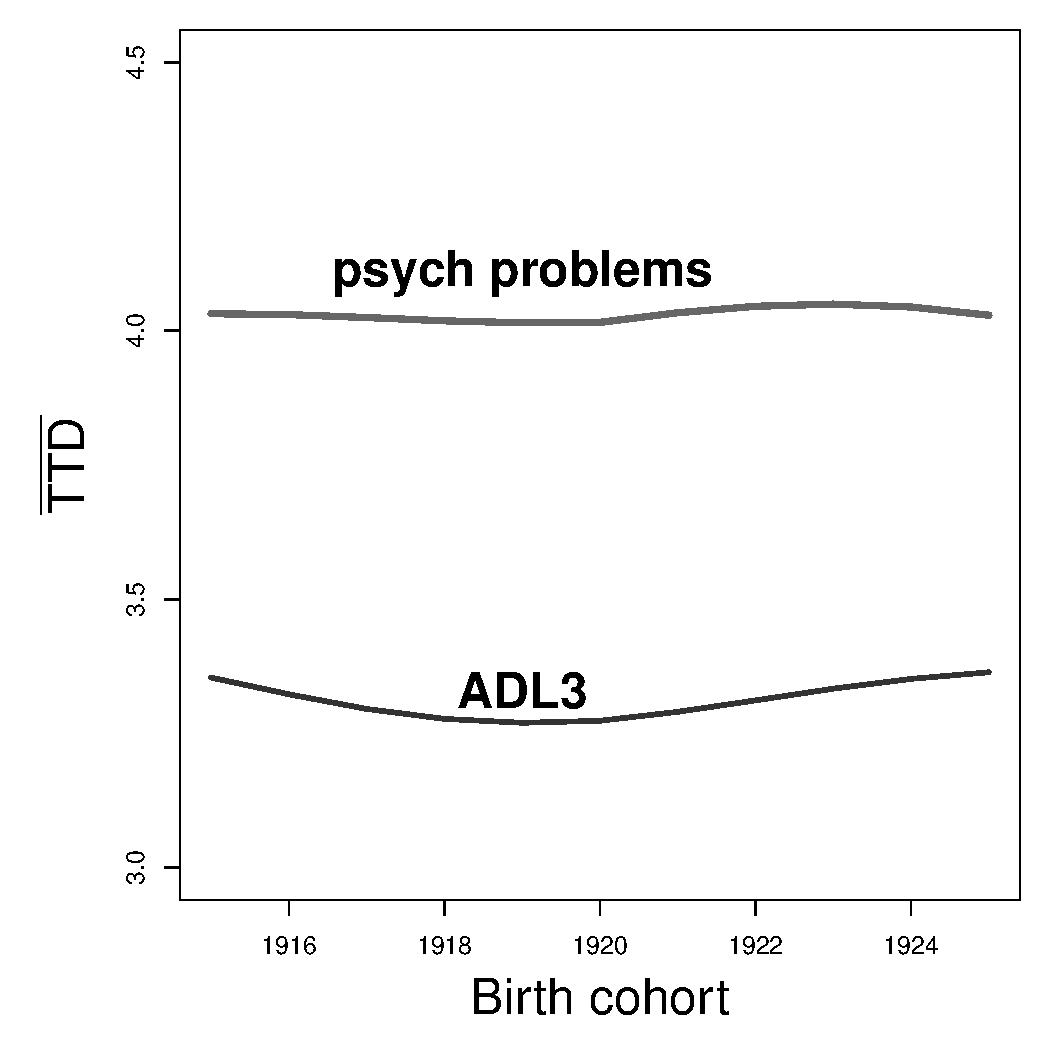
\includegraphics[scale=.9]{Figures/TrendsMeanTTD.pdf}
%\end{center}

\begin{frame}
\frametitle{Results from HRS (RAND, vP), 82 measures}

\begin{overlayarea}{\textwidth}{\textheight}
\vspace{-2em}
  \begin{columns}
    \column{0.5\textwidth}
      \centering 
      Males \\ \vspace{.5em}
      \only<1>{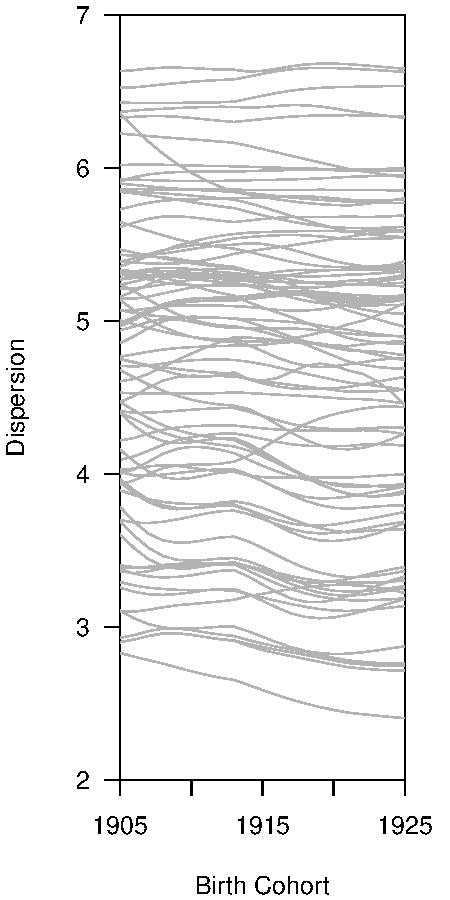
\includegraphics[height=1.1\textheight,keepaspectratio]{Figures/Mtr1.pdf}}
      \only<2>{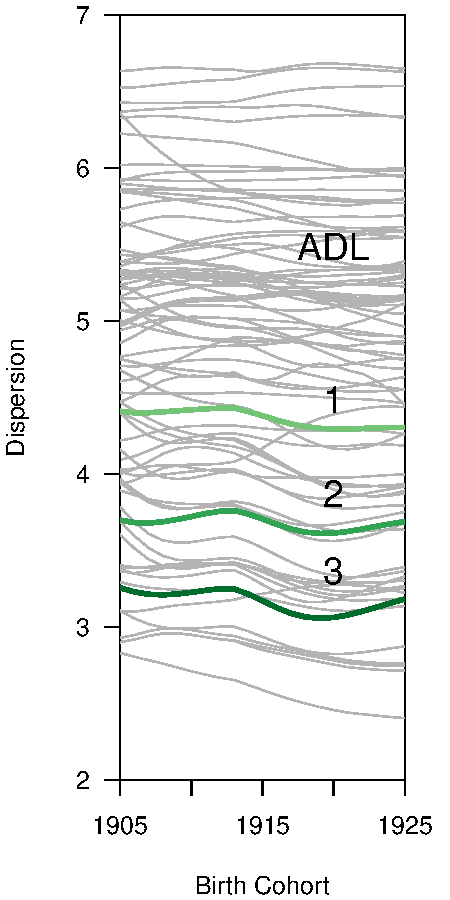
\includegraphics[height=1.1\textheight,keepaspectratio]{Figures/Mtr2.pdf}}
      \only<3>{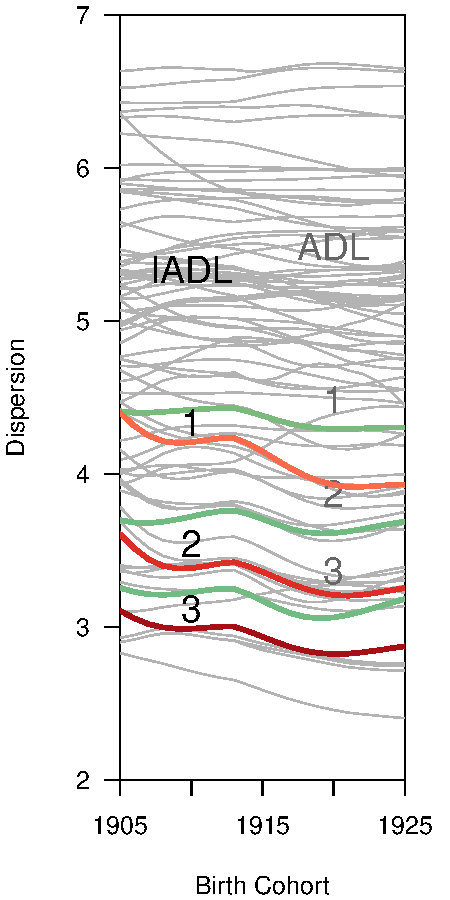
\includegraphics[height=1.1\textheight,keepaspectratio]{Figures/Mtr3.pdf}}
    \column{0.5\textwidth}
    \centering
      Females \\ \vspace{.5em}
      \only<1>{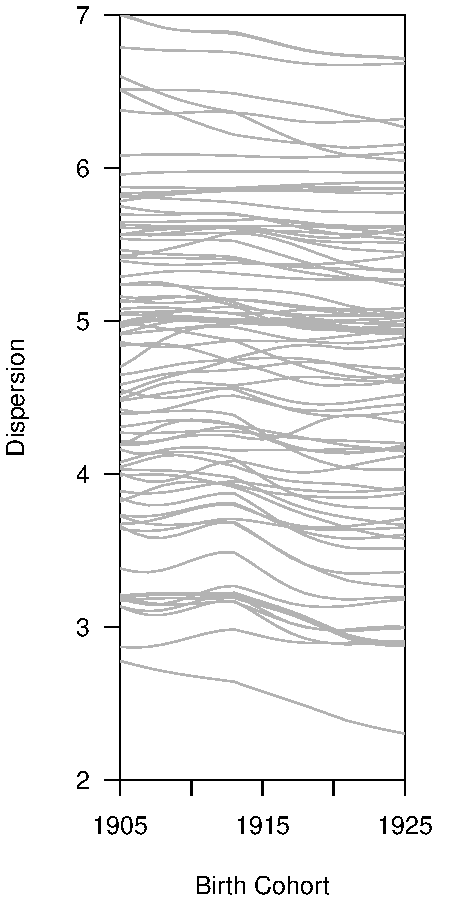
\includegraphics[height=1.1\textheight,keepaspectratio]{Figures/Ftr1.pdf}}
      \only<2>{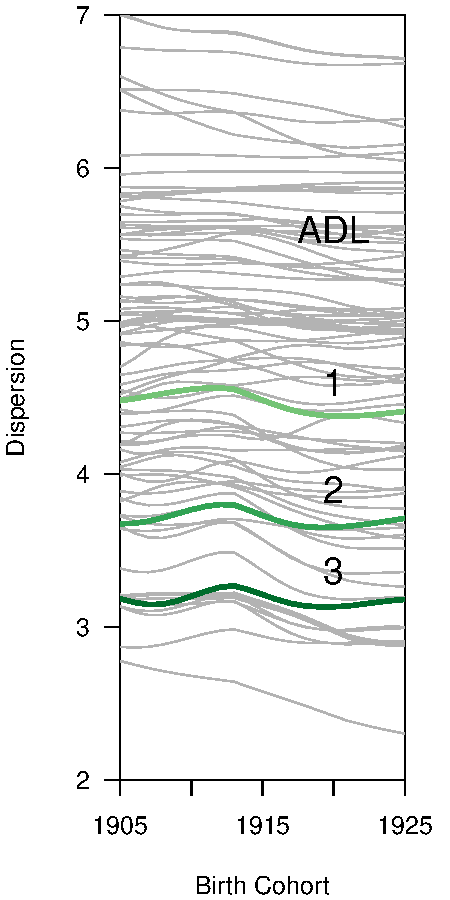
\includegraphics[height=1.1\textheight,keepaspectratio]{Figures/Ftr2.pdf}}
      \only<3>{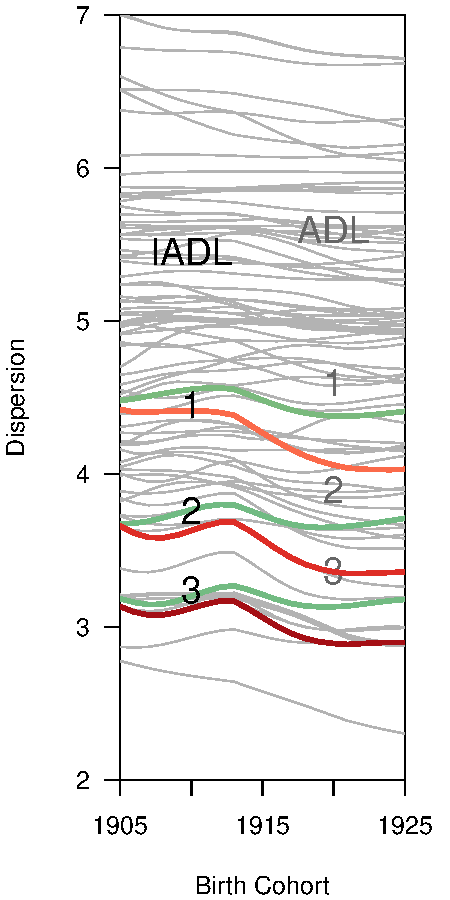
\includegraphics[height=1.1\textheight,keepaspectratio]{Figures/Ftr3.pdf}}
  \end{columns}
  \end{overlayarea}

\end{frame}

\begin{frame}
\frametitle{Summary}
\begin{block}{Measures}
Dispersion measures an aspect of the shape of morbidity prevalance, and it is a
complementary index to compression. 
\end{block}
\pause
\begin{block}{Trends}
Dispersion of most morbidities changed less than 10\% between the 1905 and 1925
cohorts, mostly in the direction of increased concetration of poor health
conditions at the end of life.
\end{block}
\pause
\begin{block}{Limitations}
This measure requires follow-up until death (but stable patterns might make
prevalance less risky to extrapolate). 
\end{block}
\end{frame}

%----------------------------------
%%%%%%%%%%%%%%%%%%%%%%%%%%%%%%%%%%
%%	End of the document			%%
%%%%%%%%%%%%%%%%%%%%%%%%%%%%%%%%%%
\end{document}










